% ============================================================
% FEE3411 Control Systems A -- Lecture notes, Week 02
% Topic: Mathematical modelling of physical systems
%
% Build:  latexmk -pdf week-02-notes.tex
% Needs:  ../tex/preamble.tex (this file lives in Notes/).
% ============================================================
\documentclass[11pt,a4paper]{article}
\usepackage[margin=25mm]{geometry}
% ============================================================
% FEE3411 Control Systems A -- shared preamble
% Used by both the lecture notes (article) and the slides (beamer).
% ============================================================
\usepackage[T1]{fontenc}
% lmodern gives cleaner PDF fonts but is absent from minimal TeX installs.
% Load it only if present, so this preamble builds anywhere.
\IfFileExists{lmodern.sty}{\usepackage{lmodern}}{}
\usepackage{amsmath,amssymb,amsthm}
\usepackage{graphicx}
\usepackage{booktabs}
\usepackage{siunitx}
\usepackage{tikz}
\usepackage{circuitikz}
\usepackage{pgfplots}
\pgfplotsset{compat=1.18}
\usetikzlibrary{arrows.meta,positioning,calc,decorations.markings,shapes.geometric}
\usepackage[most]{tcolorbox}
\usepackage{xcolor}

% ---- Course colours -------------------------------------------------
\definecolor{fnavy}{HTML}{1F3864}
\definecolor{faccent}{HTML}{2E5E4E}
\definecolor{fflag}{HTML}{9C4221}

% ---- Block-diagram style --------------------------------------------
\tikzset{
  block/.style   = {draw, thick, rectangle, minimum height=2.6em,
                    minimum width=3.2em, align=center},
  sumnode/.style = {draw, thick, circle, inner sep=0pt, minimum size=1.6em},
  pickoff/.style = {fill, circle, inner sep=0pt, minimum size=3pt},
  sig/.style     = {-{Latex[length=2mm]}, thick},
}

% ---- Summing-junction signs -----------------------------------------
% \sumsign{<node>}{<angle>}{<+ or ->} places a sign just outside the circle.
\newcommand{\sumsign}[3]{\node[font=\small] at ($(#1)+(#2:0.5)$) {$#3$};}

% ---- Boxed environments ---------------------------------------------
\newtcolorbox{keyidea}[1][]{colback=fnavy!5,colframe=fnavy,
  fonttitle=\bfseries,title=Key idea,#1}
\newtcolorbox{workedex}[1][]{colback=faccent!5,colframe=faccent,
  fonttitle=\bfseries,title=Worked example,#1}
\newtcolorbox{pitfall}[1][]{colback=fflag!5,colframe=fflag,
  fonttitle=\bfseries,title=Common pitfall,#1}

% ---- Shorthands ------------------------------------------------------
\newcommand{\Lap}{\mathcal{L}}
\newcommand{\jw}{\mathrm{j}\omega}
\newcommand{\wn}{\omega_{n}}
\newcommand{\zt}{\zeta}
\newcommand{\TF}[1]{#1(s)}

% ---- Week title machinery -------------------------------------------
\usepackage{fancyhdr}
\newcommand{\thecoursecode}{FEE3411}
\newcommand{\thecoursename}{Control Systems A}
\newcommand{\wknum}{}
\newcommand{\wktopic}{}
\newcommand{\weeknumber}[1]{\renewcommand{\wknum}{#1}}
\newcommand{\weektopic}[1]{\renewcommand{\wktopic}{#1}}
\newcommand{\weektitle}{%
  \thispagestyle{plain}%
  \begin{center}
    {\large\sffamily\bfseries\color{fnavy}\thecoursecode: \thecoursename}\\[2pt]
    {\Huge\sffamily\bfseries Week \wknum}\\[4pt]
    {\LARGE\sffamily\color{fnavy}\wktopic}\\[6pt]
    \rule{\textwidth}{1.2pt}
  \end{center}\vspace{4pt}%
  \pagestyle{fancy}\fancyhf{}%
  \fancyhead[L]{\footnotesize\color{gray}\thecoursecode\ Week \wknum\ --- \wktopic}%
  \fancyhead[R]{\footnotesize\color{gray}\thepage}%
  \renewcommand{\headrulewidth}{0.4pt}%
}

% ---- Outcomes and reading boxes -------------------------------------
\newenvironment{outcomes}
  {\begin{tcolorbox}[colback=white,colframe=fnavy!60,
      fonttitle=\bfseries,title=By the end of this week you should be able to]
   \begin{itemize}[leftmargin=*]}
  {\end{itemize}\end{tcolorbox}}

\newtcolorbox{readingbox}{colback=gray!5,colframe=gray!50,
  fonttitle=\bfseries,title=Reading}

% enumitem must NOT be loaded under beamer: it overwrites beamer's itemize
% templates and the bullet markers silently disappear. The notes (article) get
% it; the slides (beamer) use beamer's own list machinery instead.
\makeatletter
\@ifclassloaded{beamer}{}{\usepackage{enumitem}}
\makeatother


\weeknumber{2}
\weektopic{Mathematical Modelling of Physical Systems}

\begin{document}
\weektitle

% --------------------------------------------------------------------
\section*{What this week covers}

\begin{outcomes}
\item State the standard differential-equation model of a linear, time-invariant,
      causal (LTI) system, and write down its characteristic equation directly
      from the equation of motion.
\item Derive the governing differential equation of an electrical network from
      Kirchhoff's voltage law, and obtain its transfer function.
\item Derive the governing differential equation of a translational mechanical
      system from Newton's second law, using a free-body diagram, and recognise
      the force--voltage analogy with an electrical network.
\item Derive the governing equation of a rotational mechanical system (moment
      of inertia, torsional spring, viscous friction) by the rotational analogue
      of Newton's second law.
\item Explain how a gear train reflects torque, speed and moment of inertia
      from one shaft to another, and compute an equivalent inertia at a chosen
      shaft.
\item Derive the transfer function of an armature-controlled d.c.\ servomotor
      from first principles, with and without armature inductance, and combine
      it with a gear train driving a load.
\item Linearise a nonlinear differential equation about an operating point by a
      first-order Taylor expansion, and identify when the approximation is and
      is not valid.
\end{outcomes}

\begin{readingbox}
\textbf{Primary} --- Khalil, \S2-1 (p.~10); \S2-2.1 Electric Circuits (p.~14);
\S2-2.2 Mechanical Systems (p.~24); \S2-2.3 Electromechanical Systems (p.~37);
\S2-4 Linearization (p.~50).\\
\textbf{Secondary} --- Nise (6th ed.), \S2.4 Electrical Network Transfer
Functions (p.~47); \S2.5 Translational Mechanical System Transfer Functions
(p.~61); \S2.6 Rotational Mechanical System Transfer Functions (p.~69); \S2.7
Transfer Functions for Systems with Gears (p.~74); \S2.8 Electromechanical
System Transfer Functions (p.~79); \S2.10--2.11 Linearization (pp.~88--89).\\
\textbf{Further} --- Sundararajan, Ch.~3, Ch.~4, \S6.4.
\end{readingbox}

\noindent
\emph{Contact hours this week:} 2\,h lecture $+$ 1\,h tutorial.\\
\emph{Syllabus items addressed:} ``Inputs, plant and outputs\ldots\ Mathematical
models. The characteristic equation. Linear approximation to nonlinear systems.
Analysis of linear (causal) systems\ldots'' (Time Domain Linear Systems
Analysis).\\
\emph{Expected learning outcomes:} ELO~1 --- \emph{describe the working
principles of a given control system} (the servomotor, continued from
Week~1); ELO~2 --- \emph{analyse a control system solution in the time- and
frequency-domains} (begins properly this week).

\bigskip
\noindent
\textbf{A note on the two halves.} The first lecture hour builds the general
framework and applies it to electrical networks. The second hour applies the
\emph{same} framework to mechanical systems, to gears, and to the
electromechanical system that combines both: the d.c.\ servomotor promised at
the end of Week~1. The tutorial hour is where the servomotor and linearisation
are drilled in worked problems; both are derived properly here so the notes
remain self-contained.

% ====================================================================
\part*{Part A --- The modelling framework, and electrical networks}
\addcontentsline{toc}{part}{Part A}

% --------------------------------------------------------------------
\section{From a physical system to a differential-equation model}
\label{sec:framework}

Every method in FEE3411 --- Routh--Hurwitz, root locus, Bode, Nyquist --- is
applied to a mathematical model, never to the physical system itself. This
week is about how that model is obtained. Whatever the physics, a model of a
single-input--single-output plant with input $u(t)$ and output $y(t)$ takes the
same general shape (Khalil, p.~10):
\begin{equation}
  a_n\,y^{(n)}(t) + a_{n-1}\,y^{(n-1)}(t) + \cdots + a_1\,\dot y(t) + a_0\,y(t)
  = b_m\,u^{(m)}(t) + \cdots + b_1\,\dot u(t) + b_0\,u(t),
  \label{eq:general-ode}
\end{equation}
a linear, constant-coefficient ordinary differential equation, where
$y^{(k)}=d^k y/dt^k$. Three words describe it precisely, and each is doing real
work:

\begin{itemize}[leftmargin=*]
\item \textbf{Linear} --- superposition holds: the response to $\alpha u_1+\beta
      u_2$ is $\alpha y_1 + \beta y_2$. Every coefficient in
      \eqref{eq:general-ode} multiplies $u$, $y$ or a derivative to the first
      power only; there is no $y^2$, no $u\dot y$, no $\sin y$.
\item \textbf{Time-invariant} --- the coefficients $a_i,b_i$ do not themselves
      depend on $t$. Delaying the input by $t_0$ simply delays the output by
      $t_0$; the system does not care what time it is.
\item \textbf{Causal} --- the output at time $t$ depends only on the input up
      to time $t$, never on the future. Every physical system is causal; it is
      listed as a property because \emph{mathematical} operators that are not
      causal (a pure differentiator applied to noisy data, for instance) turn
      up in textbooks and cannot be built.
\end{itemize}

\begin{keyidea}
Setting the input to zero in \eqref{eq:general-ode} and replacing each
$y^{(k)}$ by $s^k$ gives the \textbf{characteristic equation}
\[
  a_n s^n + a_{n-1}s^{n-1} + \cdots + a_1 s + a_0 = 0 .
\]
It depends only on the plant --- never on the input, and never on where in the
diagram you choose to call the output. Its roots govern every natural
(unforced) response the system can produce, which is why Weeks~7--12 are all,
in one way or another, about the location of these roots.
\end{keyidea}

\begin{pitfall}
Two different physical systems with the \emph{same} characteristic equation
behave identically in their dynamics --- same natural frequency, same damping,
same transient shape --- even though the physical quantities, the units and
the steady-state gain can be completely different. You will meet exactly this
pairing in \S\ref{sec:mech-trans} below, and it is the reason the same
mathematics serves electrical, mechanical, thermal and fluid systems alike.
\end{pitfall}

Three routes lead to a model of this form (Khalil, p.~6, revisited from
Week~1): first-principles physical laws, identification from measured
input--output data, or a combination of the two. This week is entirely about
the first route, which is the one used throughout FEE3411.

% --------------------------------------------------------------------
\section{Modelling electrical networks}
\label{sec:electrical}

\subsection{Kirchhoff's laws as the starting point}

Every lumped electrical network is modelled by two laws and three element
relations. \textbf{Kirchhoff's voltage law (KVL)}: the signed sum of voltages
round any closed loop is zero. \textbf{Kirchhoff's current law (KCL)}: the
signed sum of currents into any node is zero. The element relations, for a
resistor, inductor and capacitor with current $i(t)$ and voltage $v(t)$ in the
passive sign convention, are
\begin{equation}
  v_R = Ri, \qquad v_L = L\frac{di}{dt}, \qquad i_C = C\frac{dv_C}{dt} .
  \label{eq:elements}
\end{equation}

\begin{keyidea}
Writing KVL (or KCL) around a network with the element relations
\eqref{eq:elements} substituted in \emph{is} the differential-equation model.
No new physics is needed anywhere in this unit for an electrical network ---
only bookkeeping.
\end{keyidea}

\subsection{Worked example: the series \emph{RLC} network}
\label{sec:rlc}

\begin{figure}[htbp]
\centering
\begin{circuitikz}[scale=1.0, every node/.style={font=\small}]
\draw (0,0) to[R=$R$] (2.6,0) to[L=$L$] (5.2,0);
\draw (5.2,0) to[C, l_=$C$] (5.2,-2.2);
\draw (5.2,-2.2) -- (0,-2.2);
\draw (0,0) to[open, v^<=$v_i(t)$] (0,-2.2);
\draw[thick] (6.5,-0.1) -- (6.5,0.1);
\draw[thick] (6.5,-2.3) -- (6.5,-2.1);
\draw (5.2,0) -- (6.5,0);
\draw (5.2,-2.2) -- (6.5,-2.2);
\draw (6.5,0) to[open, v^>=$v_o(t)$] (6.5,-2.2);
\end{circuitikz}
\caption{Series $RLC$ network with source voltage $v_i(t)$ and the capacitor
voltage $v_o(t)$ taken as output. Cf.\ Khalil Fig.~2-4, p.~17, relabelled with
output $v_o$ across $C$ rather than the loop current.}
\label{fig:rlc}
\end{figure}

\begin{workedex}[title=Worked example 2.1 --- series $RLC$ network]
In Figure~\ref{fig:rlc} the same current $i(t)$ flows through all three
elements, so KVL round the loop gives
\[
  v_i(t) = Ri(t) + L\frac{di(t)}{dt} + v_o(t), \qquad i(t)=C\frac{dv_o(t)}{dt}.
\]
Substituting the second relation into the first to eliminate $i$,
\begin{equation}
  \boxed{\;LC\,\ddot v_o(t) + RC\,\dot v_o(t) + v_o(t) = v_i(t)\;}
  \label{eq:rlc-ode}
\end{equation}
a second-order linear ODE of exactly the form \eqref{eq:general-ode}. Taking
Laplace transforms with zero initial conditions,
\begin{equation}
  \frac{V_o(s)}{V_i(s)} = \frac{1}{LCs^2+RCs+1},
  \qquad\text{characteristic equation } LCs^2+RCs+1=0 .
  \label{eq:rlc-tf}
\end{equation}
For $R=\SI{6}{\ohm}$, $L=\SI{2}{\henry}$, $C=\SI{0.05}{\farad}$: $LC=0.1$,
$RC=0.3$, so $0.1s^2+0.3s+1=0$, i.e.\ $s^2+3s+10=0$, with roots
$s=-1.5\pm j2.78$.
\end{workedex}

\begin{pitfall}
Writing KVL with the \emph{wrong} variable eliminated is the commonest slip.
Decide at the outset which physical quantity is the output --- here $v_o$, the
capacitor voltage --- and eliminate every other variable ($i$ in this case) in
its favour, rather than leaving a mixed equation in both $i$ and $v_o$ that
cannot be read off against \eqref{eq:general-ode}.
\end{pitfall}

Exactly the same method handles any network with more elements or more loops:
write KVL (or KCL) for each independent loop (or node), use the element
relations to reduce to one variable, and eliminate. A network with an
operational amplifier is handled the same way, using the two ideal op-amp
conditions (zero input current, equal input voltages) in place of one of the
KCL equations. We do not need this generality in FEE3411 --- the tutorial and
Assignment~1 stay with single-loop networks --- but it is worth knowing the
method has no dead ends.

\begin{keyidea}
Next week you will meet a shortcut: replacing each element by its
\emph{impedance} ($R$, $Ls$, $1/Cs$) and applying Kirchhoff's laws directly in
the $s$-domain, which reaches \eqref{eq:rlc-tf} without ever writing a
differential equation. That is a Week~3 tool (transfer functions and the
$s$-plane); this week the differential equation is the point, because the
characteristic equation is defined from it directly.
\end{keyidea}

% ====================================================================
\part*{Part B --- Mechanical systems, gears and the d.c.\ servomotor}
\addcontentsline{toc}{part}{Part B}

% --------------------------------------------------------------------
\section{Translational mechanical systems}
\label{sec:mech-trans}

The three basic elements are the spring, the viscous damper and the mass
(Khalil, p.~24). With displacement $x(t)$ measured from an equilibrium
position and applied force $f(t)$:
\begin{equation}
  f_{\text{spring}} = Kx, \qquad
  f_{\text{damper}} = B\dot x, \qquad
  f_{\text{net}} = M\ddot x,
  \label{eq:mech-elements}
\end{equation}
where $K$ is the spring constant, $B$ the viscous friction (damping)
coefficient, and $M$ the mass. A free-body diagram --- every force acting on
the mass, drawn with its correct sign --- turns \eqref{eq:mech-elements} into
an equation of motion by Newton's second law.

\begin{figure}[htbp]
\centering
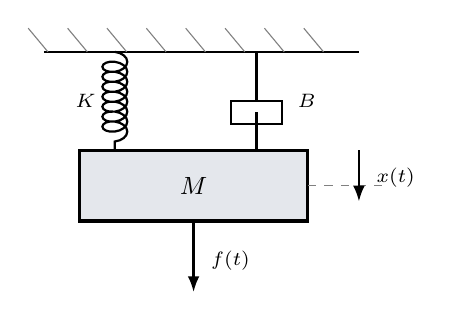
\begin{tikzpicture}[x=1cm,y=1cm,font=\small]
\draw[thick] (-0.6,0.9) -- (3.4,0.9);
\foreach \i in {0,...,7}
  \draw[gray] ({-0.55+\i*0.5},0.9) -- ({-0.8+\i*0.5},1.2);
\draw[thick, decorate, decoration={coil, aspect=0.6, segment length=3.6pt,
      amplitude=4.5pt}] (0.3,0.9) -- (0.3,-0.35);
\node[left,font=\scriptsize] at (0.18,0.28) {$K$};
\draw[thick] (2.1,0.9) -- (2.1,0.28);
\draw[thick] (1.78,0.28) rectangle (2.42,-0.02);
\draw[thick] (2.1,0.13) -- (2.1,-0.35);
\node[right,font=\scriptsize] at (2.5,0.28) {$B$};
\draw[very thick,fill=fnavy!12] (-0.15,-1.25) rectangle (2.75,-0.35);
\node at (1.3,-0.8) {$M$};
\draw[sig] (1.3,-1.25) -- (1.3,-2.15);
\node[right,font=\scriptsize] at (1.4,-1.75) {$f(t)$};
\draw[dashed,gray] (2.75,-0.8) -- (3.7,-0.8);
\draw[sig] (3.4,-0.35) -- (3.4,-1.0);
\node[right,font=\scriptsize] at (3.5,-0.7) {$x(t)$};
\end{tikzpicture}
\hspace{1.2cm}
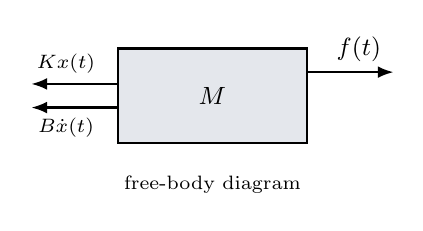
\begin{tikzpicture}[x=1cm,y=1cm,font=\small]
\draw[thick,fill=fnavy!12] (0,0) rectangle (2.4,1.2);
\node at (1.2,0.6) {$M$};
\draw[sig] (2.4,0.9) -- (3.5,0.9) node[above,pos=0.6]{$f(t)$};
\draw[sig] (0,0.75) -- (-1.1,0.75) node[above,pos=0.6,font=\scriptsize]{$Kx(t)$};
\draw[sig] (0,0.45) -- (-1.1,0.45) node[below,pos=0.6,font=\scriptsize]{$B\dot x(t)$};
\node[below] at (1.2,-0.3) {\scriptsize free-body diagram};
\end{tikzpicture}
\caption{Mass--spring--damper system and its free-body diagram: the spring and
damper forces oppose the applied force $f(t)$. Cf.\ Khalil Fig.~2-13/2-14,
p.~24, and Nise Fig.~2.15, p.~63.}
\label{fig:msd}
\end{figure}

\begin{workedex}[title=Worked example 2.2 --- mass--spring--damper]
In Figure~\ref{fig:msd} the spring and damper forces oppose the motion, so
Newton's second law gives
\[
  M\ddot x(t) = f(t) - B\dot x(t) - Kx(t)
  \qquad\Longrightarrow\qquad
  \boxed{\;M\ddot x(t) + B\dot x(t) + Kx(t) = f(t)\;}
\]
with transfer function and characteristic equation
\[
  \frac{X(s)}{F(s)} = \frac{1}{Ms^2+Bs+K}, \qquad Ms^2+Bs+K=0 .
\]
For $M=\SI{2}{\kilogram}$, $B=\SI{6}{\newton\second\per\metre}$,
$K=\SI{18}{\newton\per\metre}$: dividing through by $M$,
$s^2+3s+9=0$, roots $s=-1.5\pm j2.60$.
\end{workedex}

\begin{keyidea}[title=The force--voltage analogy]
Compare \eqref{eq:rlc-ode} with the boxed equation of Worked example~2.2 after
writing the electrical equation in terms of charge $q$, where $i=\dot q$:
\[
  L\ddot q + R\dot q + \tfrac{1}{C}q = v_i
  \qquad\longleftrightarrow\qquad
  M\ddot x + B\dot x + Kx = f .
\]
They are the \emph{same} equation under the correspondence
$M\leftrightarrow L$, $B\leftrightarrow R$, $K\leftrightarrow 1/C$,
$f\leftrightarrow v_i$, $x\leftrightarrow q$. This is why one body of
mathematics --- the second-order characteristic equation
$s^2+2\zeta\omega_n s+\omega_n^2$ that dominates Weeks~5 onward --- serves
electrical and mechanical engineers alike. It says nothing, however, about the
\emph{gain}: two analogous systems can have wildly different d.c.\ gains and
units. You will use this comparison directly in Assignment~1.
\end{keyidea}

% --------------------------------------------------------------------
\section{Rotational mechanical systems}
\label{sec:mech-rot}

Rotational systems follow the same pattern with torque $T(t)$, angle
$\theta(t)$, moment of inertia $J$, torsional spring constant $K$ and viscous
friction coefficient $b$ (Khalil, p.~53; Nise \S2.6, p.~69):
\begin{equation}
  T_{\text{spring}} = K\theta, \qquad
  T_{\text{damper}} = b\dot\theta, \qquad
  T_{\text{net}} = J\ddot\theta .
  \label{eq:rot-elements}
\end{equation}

\begin{figure}[htbp]
\centering
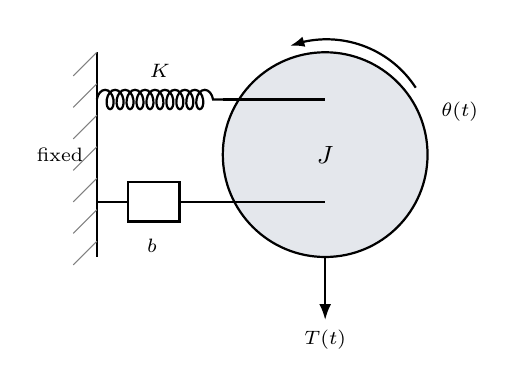
\begin{tikzpicture}[x=1cm,y=1cm,font=\small]
\draw[thick] (-0.3,1.3) -- (-0.3,-1.3);
\foreach \y in {-1.1,-0.7,-0.3,0.1,0.5,0.9,1.3}
  \draw[gray] (-0.3,\y) -- (-0.6,\y-0.3);
\draw[thick, decorate, decoration={coil, aspect=0.6, segment length=3.6pt,
      amplitude=3.5pt}] (-0.3,0.7) -- (1.3,0.7);
\node[above,font=\scriptsize] at (0.5,0.85) {$K$};
\draw[thick] (-0.3,-0.6) -- (0.1,-0.6);
\draw[thick] (0.1,-0.85) rectangle (0.75,-0.35);
\draw[thick] (0.75,-0.6) -- (1.3,-0.6);
\node[below,font=\scriptsize] at (0.4,-0.95) {$b$};
\draw[thick,fill=fnavy!12] (2.6,0) circle (1.3);
\node at (2.6,0) {$J$};
\draw[thick] (1.3,0.7) -- (2.6,0.7);
\draw[thick] (1.3,-0.6) -- (2.6,-0.6);
\draw[thick,-{Latex[length=1.8mm]}] (3.75,0.85) arc (33:110:1.35 and 1.35);
\node[right,font=\scriptsize] at (3.95,0.55) {$\theta(t)$};
\draw[sig] (2.6,-1.3) -- (2.6,-2.1) node[below,font=\scriptsize]{$T(t)$};
\node[left,font=\scriptsize] at (-0.35,0) {fixed};
\end{tikzpicture}
\caption{Rotational system: a torsional spring (represented here by the coiled
support) and viscous friction $b$ restrain an inertia $J$ driven by an applied
torque $T(t)$. Cf.\ Nise Fig.~2.21, p.~69.}
\label{fig:rot}
\end{figure}

\begin{workedex}[title=Worked example 2.3 --- rotational system]
By the rotational form of Newton's second law, with the spring and friction
torques opposing the applied torque,
\[
  J\ddot\theta(t) = T(t) - b\dot\theta(t) - K\theta(t)
  \qquad\Longrightarrow\qquad
  \boxed{\;J\ddot\theta(t)+b\dot\theta(t)+K\theta(t)=T(t)\;}
\]
\[
  \frac{\theta(s)}{T(s)}=\frac{1}{Js^2+bs+K}.
\]
When there is no restraining spring ($K=0$) --- the case of a motor shaft
driving a free inertia, met again in \S\ref{sec:servo} below --- this reduces
to $J\ddot\theta+b\dot\theta=T$, i.e.\ $\theta(s)/T(s)=1/[s(Js+b)]$: an
integrator in series with a first-order lag, the shape flagged in Week~1
equation~(6) and met repeatedly from here on.
\end{workedex}

% --------------------------------------------------------------------
\section{Gear trains}
\label{sec:gears}

A gear train couples two shafts turning at different speeds and torques. Two
meshed gears with $N_1$ and $N_2$ teeth turn through angles related by
$N_1\theta_1=N_2\theta_2$ (the teeth that mesh must match), so with
$n\triangleq\theta_2/\theta_1=N_1/N_2$ the speeds are in ratio $n$ while, since
power is conserved across an ideal (lossless) gear pair, the torques are in the
inverse ratio $T_2/T_1=1/n$ (Khalil, p.~35; Nise Fig.~2.27, p.~74).

\begin{figure}[htbp]
\centering
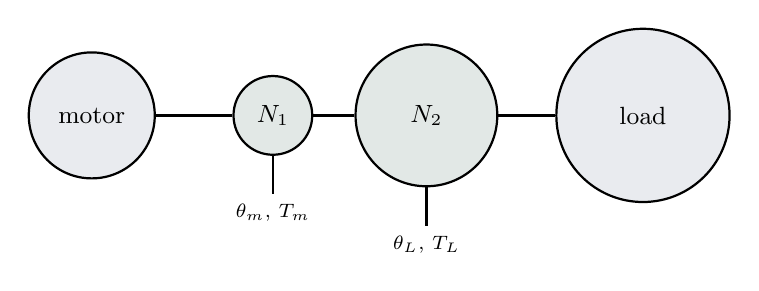
\begin{tikzpicture}[x=1cm,y=1cm,font=\small]
\node[draw,thick,circle,minimum size=1.6cm,fill=fnavy!10] (m) at (0,0) {motor};
\node[draw,thick,circle,minimum size=1.0cm,fill=faccent!14] (g1) at (2.3,0) {$N_1$};
\node[draw,thick,circle,minimum size=1.8cm,fill=faccent!14] (g2) at (4.25,0) {$N_2$};
\node[draw,thick,circle,minimum size=2.2cm,fill=fnavy!10] (l) at (7.0,0) {load};
\draw[thick] (m) -- (g1);
\draw[thick] (g1) -- (g2);
\draw[thick] (g2) -- (l);
\draw[thick] (2.3,-0.5) -- (2.3,-1.0) node[below,font=\scriptsize]{$\theta_m,\,T_m$};
\draw[thick] (4.25,-0.9) -- (4.25,-1.4) node[below,font=\scriptsize]{$\theta_L,\,T_L$};
\end{tikzpicture}
\caption{A gear train: the motor drives the small gear ($N_1$ teeth), meshed
with the load's larger gear ($N_2$ teeth), so the load turns more slowly and
with more torque than the motor. Cf.\ Khalil Fig.~2-26/2-27, p.~35--36, and
Nise Fig.~2.31, p.~77 (gear train).}
\label{fig:gears}
\end{figure}

Suppose a motor of inertia $J_m$ and friction $b_m$ drives, through a gear
train of ratio $n=\theta_L/\theta_m$, a load of inertia $J_L$ and friction
$b_L$. Writing the load's own equation of motion and substituting the
torque and angle relations through the gears into the motor's equation of
motion (Khalil, p.~36, eq.~2.30) gives, after eliminating the load variables
entirely,
\begin{equation}
  \big(J_m+n^2J_L\big)\ddot\theta_m + \big(b_m+n^2b_L\big)\dot\theta_m = T_m,
  \qquad\text{i.e.}\qquad
  J_{\text{eq}}=J_m+n^2J_L,\quad b_{\text{eq}}=b_m+n^2b_L .
  \label{eq:gear-reflect}
\end{equation}

\begin{keyidea}
The load's inertia and friction are seen at the motor shaft scaled by
$n^2$, \emph{not} by $n$. This is why a modest reduction ratio makes a huge
load feel light to the motor: at $n=1/10$ a load one hundred times the motor's
own inertia contributes only as much as the motor's own inertia again.
Equation~\eqref{eq:gear-reflect} is used again, with numbers, in
\S\ref{sec:servo-gears}.
\end{keyidea}

\begin{pitfall}
The single most common numerical error with gears is reflecting inertia by $n$
instead of $n^2$. A second is inverting the ratio --- using $\theta_m/\theta_L$
where $n=\theta_L/\theta_m$ is wanted. Both errors are easy to catch: if a
reduction gear ($n<1$) makes the equivalent inertia at the motor \emph{larger}
than the load's own inertia, or produces an implausibly large time constant,
the ratio has gone in the wrong direction somewhere.
\end{pitfall}

% --------------------------------------------------------------------
\section{The armature-controlled d.c.\ servomotor}
\label{sec:servo}

This is the electromechanical system promised at the end of Week~1: it
combines the electrical modelling of \S\ref{sec:electrical} with the
rotational modelling of \S\ref{sec:mech-rot}, coupled by the motor's two
electromechanical constants.

\begin{figure}[htbp]
\centering
\begin{circuitikz}[scale=0.95, every node/.style={font=\small}]
\draw (0,0) to[R=$R_a$] (2.2,0) to[L=$L_a$] (4.2,0);
\draw (4.2,0) to[short] (5.2,0);
\draw (0,0) to[open,v^<=$v_a(t)$] (0,-2.0);
\draw (0,-2.0) -- (5.2,-2.0);
\draw (5.2,0) to[open, i=$i_a(t)$] (5.2,0);
\node[draw,circle,minimum size=1.0cm] (bemf) at (6.3,-1.0) {$e_b$};
\draw (5.2,0) -- (6.3,-0.5); \draw (6.3,-1.5) -- (5.2,-2.0);
\draw[thick,-{Latex[length=1.8mm]}] (7.3,-1.0) arc (0:75:0.9 and 0.9);
\node[right,font=\scriptsize] at (7.5,-0.4) {$\theta_m(t)$};
\draw[thick,fill=faccent!14] (8.4,-1.0) circle (0.65);
\node[font=\scriptsize] at (8.4,-1.0) {$J_m,b$};
\draw[thick] (6.95,-1.0) -- (7.75,-1.0);
\end{circuitikz}
\caption{Armature-controlled d.c.\ servomotor: the armature circuit
($R_a$, $L_a$) drives the rotor (inertia $J_m$, friction $b$) against its own
back e.m.f.\ $e_b$; the field is separately excited and held constant. Cf.\
Khalil Fig.~2-29, p.~37, and Nise Fig.~2.35, p.~79.}
\label{fig:dcmotor}
\end{figure}

\subsection{The two coupled equations}

With armature resistance $R_a$, inductance $L_a$, current $i_a(t)$ and applied
voltage $v_a(t)$, and rotor moment of inertia $J_m$ and viscous friction $b$,
two equations describe the motor:

\paragraph{Electrical (KVL round the armature circuit).}
\begin{equation}
  v_a(t) = R_a i_a(t) + L_a\frac{di_a(t)}{dt} + e_b(t),
  \qquad e_b(t) = K_b\frac{d\theta_m(t)}{dt},
  \label{eq:motor-elec}
\end{equation}
where $e_b$ is the \textbf{back e.m.f.}, induced because a rotating armature
in a magnetic field generates a voltage opposing the current that drives it;
$K_b$ is the back-e.m.f.\ constant.

\paragraph{Mechanical (Newton's second law for rotation).}
\begin{equation}
  T_m(t) = K_t\,i_a(t) = J_m\frac{d^2\theta_m(t)}{dt^2}+b\frac{d\theta_m(t)}{dt},
  \label{eq:motor-mech}
\end{equation}
where $T_m$ is the torque developed by the motor and $K_t$ is the torque
constant.

\begin{keyidea}[title=Why this model is linear]
Two physical assumptions make \eqref{eq:motor-elec}--\eqref{eq:motor-mech}
linear, and both are worth naming explicitly rather than taking for granted:
\textbf{(i)} the field flux is held \emph{constant}, so developed torque is
directly proportional to armature current, $T_m=K_ti_a$, with no product of
two varying quantities; and \textbf{(ii)} friction is purely \emph{viscous}
(proportional to speed) --- Coulomb friction and stiction, which are not
linear, are neglected.
\end{keyidea}

\subsection{Eliminating the current: the transfer function}

Taking Laplace transforms of \eqref{eq:motor-elec}--\eqref{eq:motor-mech} with
zero initial conditions,
\[
  V_a(s) = (R_a+L_as)I_a(s) + K_bs\,\theta_m(s), \qquad
  K_tI_a(s) = (J_ms^2+bs)\theta_m(s) .
\]
The second equation gives $I_a(s)=(J_ms+b)s\,\theta_m(s)/K_t$; substituting
into the first and collecting terms in $\theta_m$,
\begin{equation}
  \boxed{\;\frac{\theta_m(s)}{V_a(s)} =
   \frac{K_t}{s\big[(R_a+L_as)(J_ms+b)+K_tK_b\big]}\;}
  \label{eq:motor-full}
\end{equation}
Note the free $s$ standing outside the bracket: it was factored out of
$J_ms^2+bs$, and it means the motor is an \textbf{integrator} --- a constant
armature voltage produces a constant \emph{speed}, and position is the
integral of speed. This is exactly the $K/[s(\tau s+1)]$ shape flagged for the
a.c.\ servomotor in Week~1.

\subsection{The reduced form: negligible armature inductance}

Armature inductance is usually small enough to neglect for control purposes.
Setting $L_a=0$ in \eqref{eq:motor-full}:
\[
  \frac{\theta_m}{V_a} = \frac{K_t}{s\big[R_a(J_ms+b)+K_tK_b\big]}
  = \frac{K_t/(R_ab+K_tK_b)}
        {s\Big[\dfrac{J_mR_a}{R_ab+K_tK_b}\,s+1\Big]}
\]
\begin{equation}
  \boxed{\;\frac{\theta_m(s)}{V_a(s)}=\frac{K_m}{s(\tau_ms+1)}\;},
  \qquad
  K_m=\frac{K_t}{R_ab+K_tK_b}, \qquad
  \tau_m=\frac{J_mR_a}{R_ab+K_tK_b} .
  \label{eq:motor-reduced}
\end{equation}

\begin{pitfall}
Khalil's textbook treatment (\S2-2.3, eq.~2.31) goes one step further and also
sets the motor's own bearing friction $b\to0$, giving the simpler
$K_m=1/K_b$, $\tau_m=J_mR_a/(K_tK_b)$. That extra simplification is \emph{not}
made in \eqref{eq:motor-reduced} above, nor in Assignment~1: the motor's own
friction $b$ is kept, because in practice $K_tK_b$ (the electromechanical
damping from the back e.m.f.) dominates $R_ab$ but does not always render it
negligible. Check which simplification a question wants before quoting a
formula from memory.
\end{pitfall}

\begin{workedex}[title=Worked example 2.4 --- servomotor constants]
For $R_a=\SI{5}{\ohm}$, $K_t=\SI{0.6}{\newton\metre\per\ampere}$,
$K_b=\SI{0.6}{\volt\second\per\radian}$, $J_m=\SI{0.01}{\kilogram\metre\squared}$
and $b=\SI{0.02}{\newton\metre\second\per\radian}$:
\[
  R_ab+K_tK_b = (5)(0.02)+(0.6)(0.6) = 0.1+0.36 = 0.46,
\]
\[
  K_m=\frac{0.6}{0.46}=\SI{1.30}{\radian\per\volt\per\second}, \qquad
  \tau_m=\frac{(0.01)(5)}{0.46}=\SI{0.109}{\second} .
\]
As in Assignment~1, notice how much of the denominator comes from $K_tK_b$
rather than from $R_ab$: the motor's own back e.m.f.\ supplies most of its
damping, exactly as observed for the a.c.\ servomotor in Week~1.
\end{workedex}

\subsection{Driving a load through a gear train}
\label{sec:servo-gears}

Combine \S\ref{sec:gears} with the servomotor: if the motor drives a load of
inertia $J_L$ through a gear train of ratio $n=\theta_L/\theta_m$, and load
friction is negligible, then by \eqref{eq:gear-reflect} the load contributes an
additional $n^2J_L$ at the motor shaft, so every occurrence of $J_m$ in
\eqref{eq:motor-reduced} is simply replaced by
\begin{equation}
  J_{\text{eq}} = J_m + n^2J_L .
  \label{eq:servo-gear-Jeq}
\end{equation}

\begin{workedex}[title=Worked example 2.5 --- geared servomotor]
Take the motor of Worked example~2.4, now driving a load
$J_L=\SI{2}{\kilogram\metre\squared}$ through a gear train of ratio
$n=1/5$. Then
\[
  J_{\text{eq}} = 0.01 + \left(\tfrac{1}{5}\right)^2(2) = 0.01+0.08
   = \SI{0.09}{\kilogram\metre\squared},
\]
\[
  \tau_m' = \frac{J_{\text{eq}}R_a}{R_ab+K_tK_b} = \frac{(0.09)(5)}{0.46}
   = \SI{0.978}{\second},
\]
roughly nine times slower than the unloaded motor of Worked example~2.4. Note
how effective the gearing still is: without it ($n=1$) the equivalent inertia
would be $2.01\,\si{\kilogram\metre\squared}$ and $\tau_m$ over
\SI{21}{\second} --- far too sluggish for a servo.
\end{workedex}

% --------------------------------------------------------------------
\section{Linear approximation to nonlinear systems}
\label{sec:linearization}

Real components are rarely linear over their whole operating range: a spring
stiffens as it is compressed, a valve's flow is not proportional to its
opening, a motor saturates. Yet almost every method in this unit assumes
\eqref{eq:general-ode}. \textbf{Linearization} is what bridges the gap
(Khalil, p.~50; Nise \S2.11, p.~89).

\begin{keyidea}
Near an operating (equilibrium) point, a smooth nonlinear function can be
replaced by the tangent line at that point: a first-order Taylor expansion.
The approximation is good \emph{only} for small excursions about that point,
and a linearization performed about one operating point does not, in general,
apply near a different one.
\end{keyidea}

For a static nonlinearity $y=f(x)$ about operating point $(x_0,y_0)$, with
$y_0=f(x_0)$,
\begin{equation}
  \Delta y \;\approx\; f'(x_0)\,\Delta x, \qquad \Delta x = x-x_0,\quad
  \Delta y = y-y_0 .
  \label{eq:lin-static}
\end{equation}
This is precisely the method already used, without naming it, for the a.c.\
servomotor torque--speed characteristic in Week~1: $T_m=f(\dot\theta,E)$ was
expanded about an operating point to give
$\Delta T_m=K\Delta E-f\Delta\dot\theta$.

For a \emph{dynamic} system $\dot x=f(x,u)$, linearization is done about an
equilibrium point $(x_0,u_0)$ satisfying $f(x_0,u_0)=0$ --- a point where the
system, once there, stays there with no input change --- using the same
first-order Taylor idea on each variable.

\begin{figure}[htbp]
\centering
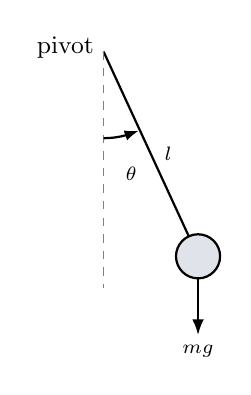
\begin{tikzpicture}[x=1cm,y=1cm,font=\small]
\draw[thick] (0,0) -- (1.2,-2.6);
\draw[thick,fill=fnavy!14] (1.2,-2.6) circle (0.28);
\node[left] at (0,0.05) {pivot};
\draw[dashed,gray] (0,0) -- (0,-3.0);
\draw[thick,-{Latex[length=1.8mm]}] (0,-1.1) arc (270:294:1.1);
\node[font=\scriptsize] at (0.35,-1.55) {$\theta$};
\node[right,font=\scriptsize] at (0.65,-1.3) {$l$};
\draw[sig] (1.2,-2.88) -- (1.2,-3.6) node[below,font=\scriptsize]{$mg$};
\end{tikzpicture}
\caption{The simple pendulum: rigid massless rod of length $l$, bob of mass
$m$, viscous friction coefficient $k$ (not shown) resisting the swing. Cf.\
Khalil Fig.~2-44, p.~51.}
\label{fig:pendulum}
\end{figure}

\begin{workedex}[title=Worked example 2.6 --- linearizing the pendulum]
For the pendulum of Figure~\ref{fig:pendulum}, Newton's second law in the
tangential direction (which conveniently eliminates the rod tension) gives
\[
  ml\,\ddot\theta(t) = -mg\sin\theta(t) - kl\,\dot\theta(t) .
\]
Setting $\dot\theta=\ddot\theta=0$ for equilibrium gives $\sin\theta=0$, so
$\theta=0,\pm\pi,\pm2\pi,\ldots$; only $\theta=0$ (hanging down) and
$\theta=\pi$ (balanced upright) are physically distinct.

\smallskip
\textbf{About $\theta=0$}: for small $\theta$, $\sin\theta\approx\theta$, so
\[
  \boxed{\;ml\,\ddot\theta+kl\,\dot\theta+mg\,\theta=0\;}
\]
a stable, oscillatory (or decaying) linear system --- the restoring term
$mg\theta$ opposes any displacement.

\smallskip
\textbf{About $\theta=\pi$}: writing $\theta=\pi+\phi$ for a small excursion
$\phi$, $\sin\theta=\sin(\pi+\phi)=-\sin\phi\approx-\phi$, so
\[
  \boxed{\;ml\,\ddot\phi+kl\,\dot\phi-mg\,\phi=0\;} .
\]
The sign of the $\phi$ term has \emph{flipped}: this linear equation has a
positive root and $\phi$ grows without bound, correctly predicting that the
inverted pendulum is unstable.
\end{workedex}

\begin{pitfall}
A linearization is only valid near the point it was taken about. The two
equations in Worked example~2.6 look almost identical but describe opposite
behaviour, because they linearize about a stable and an unstable equilibrium
respectively. Quoting a linearized model without stating which operating point
it belongs to is a meaningless answer.
\end{pitfall}

% --------------------------------------------------------------------
\section*{Summary}

\begin{itemize}
\item An LTI causal system's differential-equation model always has the shape
      of equation~\eqref{eq:general-ode}; its characteristic equation depends
      only on the plant, never on the input.
\item Electrical networks are modelled by Kirchhoff's laws with the element
      relations $v_R=Ri$, $v_L=L\dot i$, $i_C=C\dot v_C$; translational
      mechanical systems by Newton's second law with $f=Kx$, $B\dot x$,
      $M\ddot x$; rotational systems the same way with torque, angle and
      moment of inertia.
\item The force--voltage analogy ($M\leftrightarrow L$, $B\leftrightarrow R$,
      $K\leftrightarrow 1/C$) means electrical and mechanical systems with the
      same characteristic equation have identical dynamics but, in general,
      different gains and units.
\item A gear train of ratio $n=\theta_2/\theta_1$ reflects torque by $1/n$ and
      inertia (and friction) by $n^2$: $J_{\text{eq}}=J_1+n^2J_2$.
\item The armature-controlled d.c.\ servomotor couples an electrical equation
      (KVL with back e.m.f.) to a mechanical one (torque balance); eliminating
      the armature current gives $\theta_m/V_a=K_t/\{s[(R_a+L_as)(J_ms+b)+K_tK_b]\}$,
      which reduces to $K_m/[s(\tau_ms+1)]$ when $L_a\to0$.
\item Linearization replaces a nonlinear equation by its first-order Taylor
      expansion about a stated operating point; the result, and even its
      stability, can differ completely between operating points.
\end{itemize}

% --------------------------------------------------------------------
\section*{Before the tutorial}

\begin{enumerate}
\item Derive the differential equation and transfer function $I(s)/V(s)$ of a
      \emph{parallel} $RLC$ network driven by a current source, with the loop
      voltage as output. Compare the form of your characteristic equation with
      equation~\eqref{eq:rlc-tf}.
\item A rotational system has $J=\SI{0.4}{\kilogram\metre\squared}$,
      $b=\SI{1.2}{\newton\metre\second\per\radian}$, and no restoring spring.
      Write its transfer function $\theta(s)/T(s)$ and identify its time
      constant.
\item A valve has flow rate $q=k\sqrt{p}$ for pressure drop $p$ across it,
      where $k$ is a constant. Linearize this relation about an operating point
      $p_0$, and state the range of $p$ over which you would trust the linear
      model.
\end{enumerate}

% --------------------------------------------------------------------
\section*{Looking ahead}

Next week takes the differential-equation models built here and passes them
through the Laplace transform to get transfer functions directly, introduces
the impedance shortcut flagged in \S\ref{sec:electrical}, and studies poles,
zeros and the pole--zero map in the $s$-plane --- the geometric picture behind
everything from Week~5 onward. Assignment~1, issued in Week~1 and due at the
start of the Week~3 lecture, sets its Questions~3 and~4 directly against this
week's material (network and mass--spring--damper modelling, and the geared
d.c.\ servomotor): attempt them now, using the method demonstrated here with
your own working, not the numbers used in the worked examples above. As
throughout FEE3411, deriving these models is \emph{analysis}; using a
linearized model to design a compensator, or handling parameter uncertainty in
the model itself, is FEE3412's business, not this unit's.

\end{document}
